% Learning Where to Sharpen
% Drafted for IIAI AAI / SCAI. Swap \documentclass for the venue template when it
% arrives; nothing below depends on IEEEtran beyond the two-column environment.
\documentclass[conference]{IEEEtran}
\IEEEoverridecommandlockouts

\usepackage{cite}
\usepackage{amsmath,amssymb}
\usepackage{graphicx}
\usepackage{booktabs}
\usepackage{url}
\usepackage{tikz}
\usetikzlibrary{arrows.meta,positioning,calc}
\usepackage[hidelinks]{hyperref}

\newcommand{\bfone}{BF\textsubscript{1}}

\begin{document}

\title{Learning Where to Sharpen: Selective Boundary\\Refinement for Diffusion-Based Monocular Depth}

\author{\IEEEauthorblockN{TODO Author}
\IEEEauthorblockA{TODO Affiliation\\
TODO email}}

\maketitle

\begin{abstract}
Diffusion-based monocular depth estimators produce accurate surfaces but blurred
depth discontinuities. A natural remedy is to sharpen the predicted depth at
contours found by a segmentation model, yet applying a barrier-sharpening
operation at every contour \emph{lowers} boundary \bfone{} by 1.90\% on NYUv2.
We show by measurement that the bottleneck is not where the contours are --- a
true depth step is a median 1.00\,px from the nearest contour --- but which
contours to use: 79.8\% of them lie where no depth step exists. Keeping only the
correct 4\% with ground truth, without moving a single contour, turns $-1.90\%$
into $+43.39\%$. We therefore fix the repair operation and learn only
\emph{where} to apply it. A 1.9M-parameter selector trained for 16 minutes on
795 frames raises \bfone{} by $11.92 \pm 0.90\%$ on NYUv2 over four seeds, and
transfers with no retraining to a second depth model of a different
architecture and output representation, raising its \bfone{} by $27.83 \pm
1.27\%$. Five training-free controls, measured on each model's own predictions,
place the learning's contribution at 10.7 and 17.4 points. The selector and the
repair add 30\,ms per frame, and a coarse segmentation grid delivers 95\% of
the gain at 20\% of the segmentation cost. We also report a negative result:
the selector transfers across depth models but not across datasets, and four
remedies failed to fix it.
\end{abstract}

\begin{IEEEkeywords}
monocular depth estimation, depth boundaries, post-processing, diffusion models
\end{IEEEkeywords}

\section{Introduction}

Monocular depth estimators built on pre-trained diffusion
models~\cite{marigold,lotus,marigoldv2} reach strong pixel-wise accuracy, but
they inherit the smoothness of the generative prior at object boundaries. A
depth map can have excellent AbsRel while every occlusion boundary in it is
spread over several pixels. Pixel-averaged metrics do not see this: the
boundary pixels are a small fraction of the image, so a metric dominated by
flat surfaces reports no problem. Boundary-specific metrics
do~\cite{depthpro}.

Fixing boundaries after the fact is attractive because it leaves the depth
model untouched. Prior work learns \emph{how} to move the
depth~\cite{ramamonjisoa,sharpnet,edgeguided}. We take the opposite
decomposition: fix the repair, and learn \emph{where} it should act.

The reason is empirical. Section~\ref{sec:diagnosis} measures a
barrier-sharpening operation applied at every contour a segmentation
model~\cite{sam} draws, and finds it \emph{costs} 1.90\% of boundary \bfone{}.
The same measurement shows why: contour localisation is already good enough,
while 79.8\% of the contours mark no depth step at all, and sharpening there
only flattens smooth surface. Selecting the correct contours with ground truth,
with no change to their positions, moves the effect from $-1.90\%$ to
$+43.39\%$. Selection, not localisation, is the binding constraint.

Our contributions:

\begin{enumerate}
\item A measurement that identifies selection as the bottleneck in post-hoc
      boundary sharpening, including an oracle that reverses the sign of the
      effect without moving any contour (Sec.~\ref{sec:diagnosis}).
\item A method that fixes the repair operation and learns only the selection, so
      that what the learning contributes is directly attributable
      (Sec.~\ref{sec:method}).
\item Results on two depth models that differ in architecture, parameter count
      and output representation, with four seeds each and five training-free
      controls measured on each model's own predictions
      (Sec.~\ref{sec:experiments}).
\item A cost analysis showing the added work is 30\,ms per frame and that a
      coarse segmentation grid gives 95\% of the gain at 20\% of the
      segmentation cost (Sec.~\ref{sec:cost}).
\end{enumerate}

We also report, in Sec.~\ref{sec:limitations}, that the selector does not
transfer across datasets, and that four attempts to fix that failed.

\begin{figure*}[t]
\centering
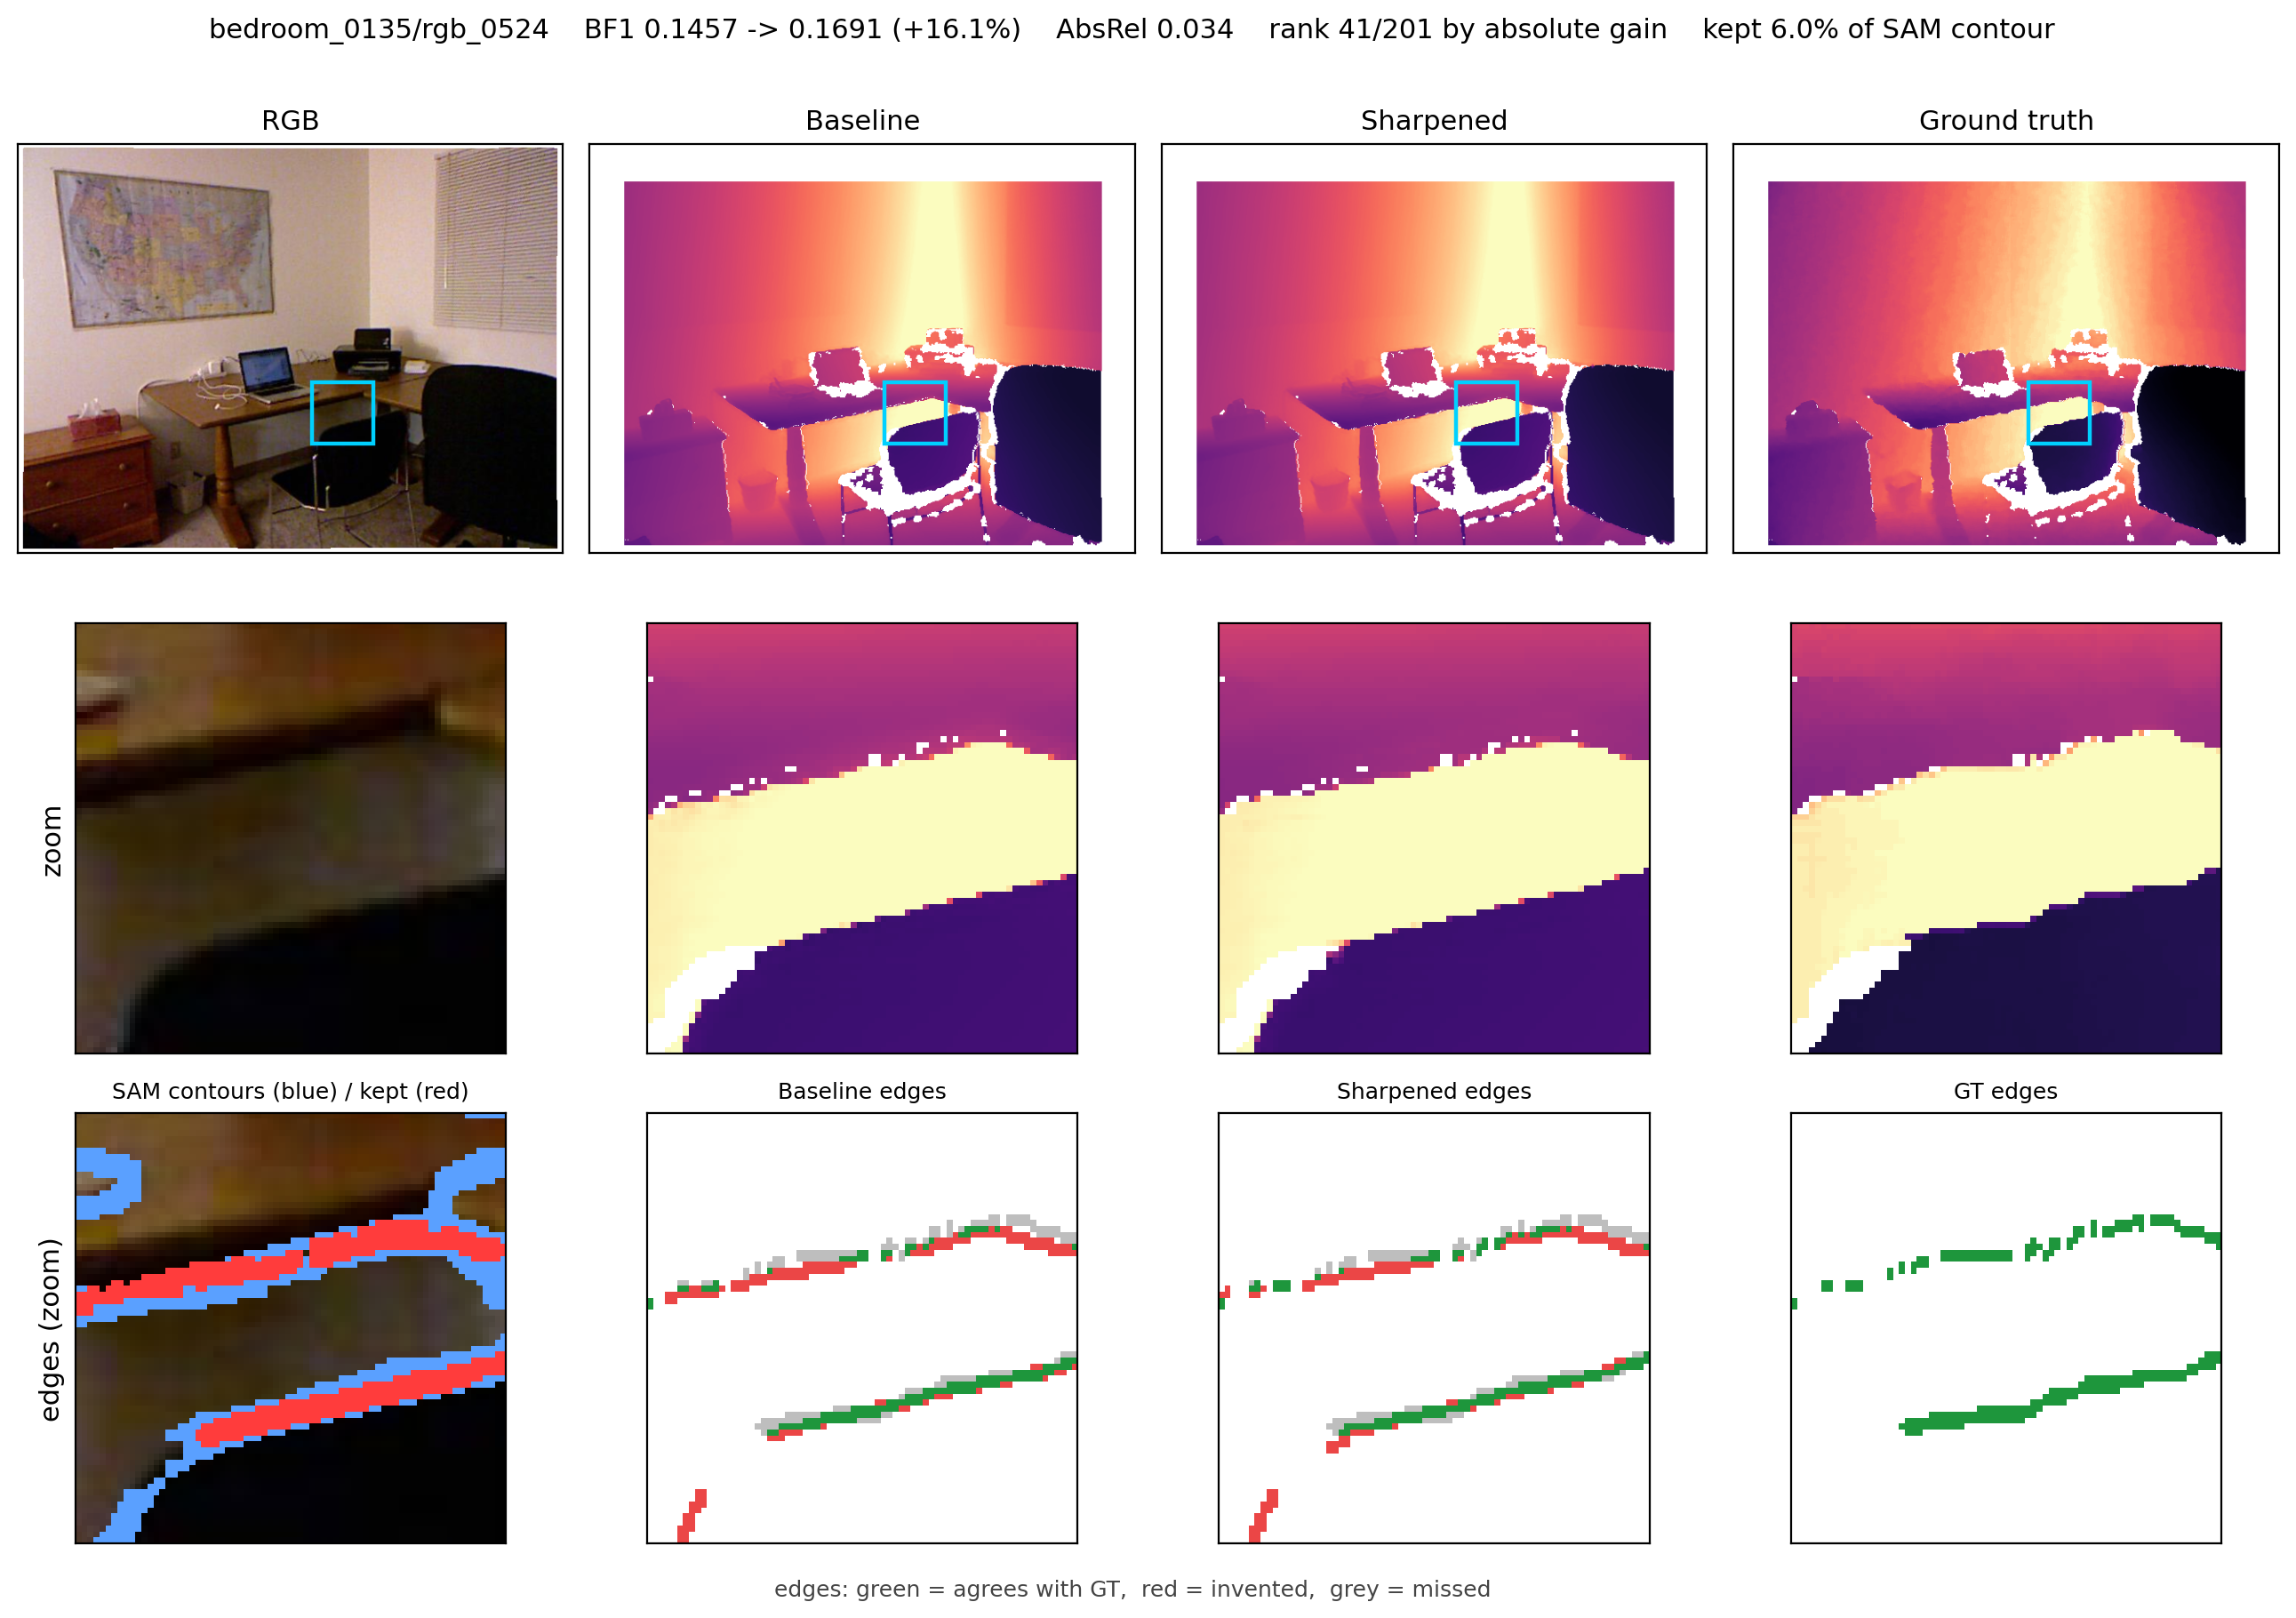
\includegraphics[width=\textwidth]{figures/qualitative_a.png}
\caption{What the method does. Top: the whole frame; nothing outside the
selected contours moves. Middle: a 72\,px crop --- the baseline's desk edge is
spread over several pixels, the sharpened map restores the step. Bottom: the
depth discontinuities each map contains, which is what \bfone{} compares; green
agrees with ground truth, red is invented, grey is missed. The panel states the
frame's AbsRel and its rank among eligible frames, so the reader can see that
this is not the best case in the split.}
\label{fig:qualitative}
\end{figure*}

\section{Related Work}

\textbf{Diffusion-based monocular depth.}
Marigold~\cite{marigold} repurposes Stable Diffusion for affine-invariant
monocular depth by fine-tuning on synthetic RGB-D. Lotus~\cite{lotus} removes
the diffusion schedule, predicting in a single step with the timestep pinned.
Subsequent work showed that one-step fine-tuning both simplifies and
accelerates these models by orders of magnitude~\cite{onestep}. We evaluate on
two such models that are as far apart as the family allows: a 21.3B
diffusion-transformer model emitting affine-invariant log depth, and an 868M
UNet model emitting disparity.

\textbf{Boundary sharpening as post-processing.}
Ramamonjisoa et al.~\cite{ramamonjisoa} is the closest prior work: it learns a
2D displacement field that re-samples pixels around occlusion boundaries, is
applicable to any depth estimator's output, and uses NYUv2 with the same 795
training and 654 test frames we use. SharpNet~\cite{sharpnet} instead builds
occluding-contour recovery into the depth network's own training.
Edge-guided post-processing~\cite{edgeguided} preserves boundaries during
disparity synthesis in self-supervised pipelines. More recently, depth
refinement through neural radiance fields~\cite{nerfrefine} reports a 2.9\%
relative improvement in edge F1. All of these learn how to move depth. None, to
our knowledge, fixes the repair and learns only its target, and none uses a
promptable segmentation model as the source of candidate boundaries.

\textbf{We do not compare directly against~\cite{ramamonjisoa}.} Its code is
public but no trained weights are released, the README documents no inference
procedure, and it requires PyTorch $\geq 0.4$, which does not run under current
PyTorch. We instead ablate our own use of segmentation
(Sec.~\ref{sec:experiments}), which answers the related question of how much
the external segmentation contributes. That is an ablation of our method, not a
comparison against prior work, and we do not present it as one.

\textbf{Boundary metrics.}
We adopt the scale-invariant boundary \bfone{} of Depth Pro~\cite{depthpro},
which declares a depth step between neighbouring pixels when their depth
\emph{ratio} exceeds a threshold, and sweeps that threshold. We propose no new
metric. Neither Lotus nor the diffusion-transformer model we use reports
\bfone{} on NYUv2, so we measure the baselines ourselves.

\textbf{Segmentation for depth.} Segment Anything~\cite{sam} has been used to
refine masks with depth as a prior; we use it in the opposite direction, as a
source of candidate depth boundaries that a learned selector then filters.

\section{Diagnosis: selection is the bottleneck}
\label{sec:diagnosis}

\subsection{The repair operation}

Let $d$ be a predicted depth map and $C$ a set of contour pixels. The
barrier-sharpening operation discards a band of $\pm 2$\,px around $C$, floods
the region labels from outside the band inward so that the two sides of a
contour meet inside it rather than one leaking across, and refills each
discarded pixel with the local mean of its \emph{own} side within a radius of
3\,px. The band is discarded because a diffusion model interpolates across the
boundary; refilling from one side only removes that mixing. The operation has
two settings and learns nothing. The refill radius must exceed the band, or
there is nothing to refill from and the operation is a silent no-op.

\subsection{Applying it everywhere fails}

Table~\ref{tab:diagnosis} applies the operation at every contour that Segment
Anything draws on NYUv2, using a 21.3B diffusion-transformer depth model as the
base. Boundary \bfone{} falls by 1.90\%.

\begin{table}[t]
\caption{Why post-hoc sharpening fails, and what fixes it. NYUv2, 654 frames.
Oracle selection uses ground truth and moves no contour.}
\label{tab:diagnosis}
\centering
\begin{tabular}{lrr}
\toprule
Contours sharpened & kept & raw \bfone{} \\
\midrule
all segmentation contours      & 100\%  & $-1.90\%$ \\
oracle: only the true ones     & 4\%    & $\mathbf{+43.39\%}$ \\
\bottomrule
\end{tabular}
\end{table}

\subsection{Localisation is not the problem}

Measuring from each true depth discontinuity to the nearest contour gives a
median of 1.00\,px, with 76.9\% within 2\,px. The contours are where the
boundaries are. The failure is in the other direction: 79.8\% of the contour
pixels sit where no depth step exists --- wallpaper patterns, floor seams,
poster edges. Sharpening there discards a band of smooth surface and refills it
from two sides that agree, which can only add noise.

\subsection{Selecting with ground truth reverses the sign}

Keeping only the 4\% of contour pixels that lie within 1\,px of a true
discontinuity, and leaving every kept contour exactly where it is, moves the raw
effect from $-1.90\%$ to $+43.39\%$ (Table~\ref{tab:diagnosis}). No contour
moves; only the set changes. This isolates selection as the binding constraint
and sets the target for a learned selector.

\section{Method}
\label{sec:method}

\begin{figure}[t]
\centering
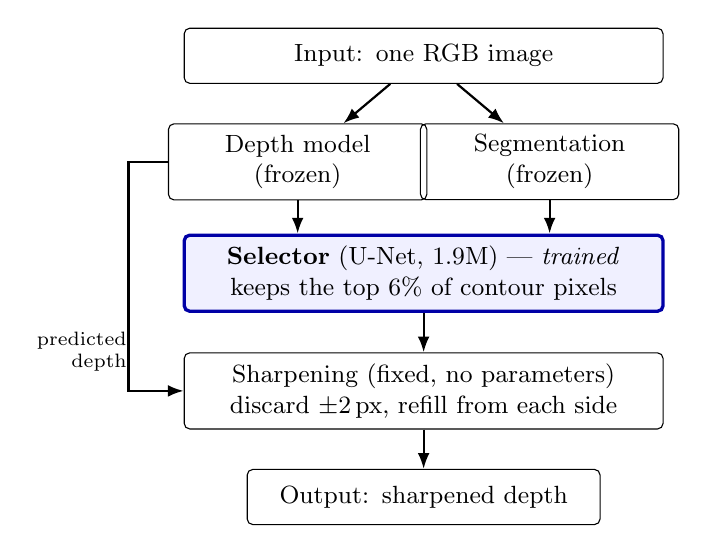
\begin{tikzpicture}[
  font=\small,
  box/.style={draw, rounded corners=2pt, align=center, inner sep=4pt,
              minimum height=7mm, text width=58mm},
  hot/.style={box, draw=blue!65!black, very thick, fill=blue!6},
  ar/.style={-{Latex[length=2mm]}, thick}
]
\node[box] (in)  {Input: one RGB image};
\node[box, below=5mm of in, xshift=-16mm, text width=30mm] (mv2)
     {Depth model\\(frozen)};
\node[box, below=5mm of in, xshift=16mm, text width=30mm] (sam)
     {Segmentation\\(frozen)};
\node[hot, below=7mm of in, yshift=-12mm] (sel)
     {\textbf{Selector} (U-Net, 1.9M) --- \emph{trained}\\
      keeps the top 6\% of contour pixels};
\node[box, below=5mm of sel] (sh)
     {Sharpening (fixed, no parameters)\\
      discard $\pm 2$\,px, refill from each side};
\node[box, below=5mm of sh, text width=42mm] (out) {Output: sharpened depth};

\draw[ar] (in) -- (mv2);
\draw[ar] (in) -- (sam);
\draw[ar] (mv2) -- (sel.north -| mv2);
\draw[ar] (sam) -- (sel.north -| sam);
\draw[ar] (sel) -- (sh);
\draw[ar] (sh)  -- (out);
\draw[ar] (mv2.west) -- ++(-5mm,0) |- (sh.west);
\node[anchor=east, font=\scriptsize, align=right] at ($(sh.west)+(-6mm,5mm)$)
     {predicted\\depth};
\end{tikzpicture}
\caption{Only the selector is trained. The depth model and the segmentation
model are frozen, and the repair is a fixed operation with no parameters, so
the gain is attributable to the selection alone.}
\label{fig:pipeline}
\end{figure}

Fig.~\ref{fig:pipeline} shows the pipeline. The depth model and the
segmentation model are frozen. The repair is the fixed operation of
Sec.~\ref{sec:diagnosis}. The only trained component is the selector.

\textbf{Inputs and output.} The selector is a four-level U-Net with 1{,}928{,}993
parameters. It takes the RGB image (3 channels), the predicted depth (1), and
the contour mask (1), and emits one logit per pixel. The prediction is
standardised per image: these models are affine-invariant, so the absolute level
and scale carry no information, and a mismatch between training and inference
here is silent. For a model that emits disparity rather than log depth we apply
$-\log d$ first, since disparity rises as depth falls and feeding it raw would
invert the signal.

\textbf{Retention.} We keep the top 6\% of contour pixels per image rather than
thresholding the probability. A fixed threshold keeps a different amount
depending on how many contours a scene happens to contain, so the budget the
repair spends would drift from frame to frame.

\textbf{Loss and training.} Binary cross-entropy masked to contour pixels; the
88\% of the image that carries no contour is not a question the selector is
asked. A contour pixel is positive if it lies within 1\,px of a depth
discontinuity in ground truth. Ground truth is used only to generate these
labels and never appears in the inference path. Training uses the 795 NYUv2
training frames with a scene-disjoint validation split, takes 16 minutes and
3.5\,GB of VRAM on one RTX 4090, and never touches the 654-frame test set.

\section{Experiments}
\label{sec:experiments}

\subsection{Setup}

We evaluate on the 654-frame NYUv2~\cite{nyuv2} test split, scene-disjoint from
the training frames. The metric is the scale-invariant boundary \bfone{} of
Depth Pro~\cite{depthpro}, swept over 11 thresholds from 5\% to 25\%. We report
the raw relative change in \bfone{} against each base model's own unsharpened
prediction. Predictions are aligned to ground truth in their own space before
scoring --- log depth for one model, disparity for the other --- and the
alignment affects every variant equally.

\subsection{Main result}

Table~\ref{tab:main} gives the result on two depth models that share no
architecture, no parameter scale and no output representation. One selector is
trained, on the first model's predictions; it is applied to the second with no
retraining, adding only the disparity-to-log-depth conversion.

\begin{table}[t]
\caption{Main result. Four seeds each; $\pm$ is one standard deviation. The
same selector is applied to both models; it was trained only on the first.}
\label{tab:main}
\centering
\begin{tabular}{lrrr}
\toprule
Base depth model & \bfone{} & no selection & + selector \\
\midrule
DiT, 21.3B, log depth & 0.0884 & $-1.90\%$  & $\mathbf{+11.92 \pm 0.90\%}$ \\
UNet, 868M, disparity & 0.0693 & $+10.31\%$ & $\mathbf{+27.83 \pm 1.27\%}$ \\
\bottomrule
\end{tabular}
\end{table}

All four seeds clear $+10\%$ on the first model, with a 95\% confidence
interval whose lower bound is $+10.49\%$. Pixel-wise accuracy does not
regress: AbsRel moves from 0.03881 to 0.03860 and $\delta_1$ from 0.97969 to
0.98000. Both changes are small, and we claim only that accuracy is not traded
for boundaries.

Per-frame scoring shows the mean is not carried by a few frames: 493 of 651
scorable frames improve (75.7\%), with a median relative gain of $+14.13\%$ and
quartiles $+0.32\%$ and $+34.38\%$. Fig.~\ref{fig:qualitative} shows a frame
near the middle of that distribution.

\subsection{Controls}

The gain could come from the sharpening rather than from the learning, or from
simply being sparse. Table~\ref{tab:controls} measures five training-free
alternatives, each on the base model's own predictions.

\begin{table}[t]
\caption{Training-free controls, measured separately on each base model.
Raw \bfone{} change.}
\label{tab:controls}
\centering
\begin{tabular}{lrr}
\toprule
Selection & DiT 21.3B & UNet 868M \\
\midrule
none (all contours)            & $-1.90\%$  & $+10.31\%$ \\
relocated (same sparsity)      & $-0.50\%$  & $-0.57\%$  \\
random pixels (same rate)      & $-20.35\%$ & $-19.70\%$ \\
random blocks (same rate)      & $-1.48\%$  & $-0.67\%$  \\
best hand-crafted threshold    & $+1.25\%$  & $+10.46\%$ \\
\midrule
\textbf{trained selector}      & $\mathbf{+11.92\%}$ & $\mathbf{+27.83\%}$ \\
\textbf{learning contributes}  & $\mathbf{10.7}$\,pt & $\mathbf{17.4}$\,pt \\
\bottomrule
\end{tabular}
\end{table}

The hand-crafted control thresholds a local descriptor of the predicted depth's
log-gradient. We select its feature by the final metric rather than by ranking
quality: over four candidates the AUC ordering and the \bfone{} ordering are
\emph{inverted}, and the feature with the worst AUC (0.801) gives the best
\bfone{} ($+1.25\%$) while the best AUC (0.876) gives the worst ($-2.59\%$). A
control chosen by a proxy metric would have been too weak, and a weak control
only flatters the method compared against it.

Random-pixel selection scores almost identically on both models
($-20.35\%$ and $-19.70\%$), as it should: that control measures a property of
the repair operation, not of the depth model.

\subsection{How much the segmentation contributes}

Removing the segmentation model entirely, so that the selector must find
boundaries itself from RGB and depth and every valid pixel is a candidate,
gives $+7.30\%$ instead of $+11.92\%$. The segmentation is therefore worth
5.19 points, 42\% of the gain. The mechanism is recall, not precision: on
segmentation contours the true steps number 1{,}221 pixels per frame and the
budget of 1{,}207 can cover 98.9\% of them, whereas counting over the whole
image there are 3{,}042 and the same budget caps recall at 39.7\%. The
segmentation earns its contribution by \emph{shrinking the target set}.

\section{Cost}
\label{sec:cost}

Table~\ref{tab:cost} gives wall-clock time per frame on one RTX 4090, measured
after warm-up on real frames.

\begin{table}[t]
\caption{Per-frame cost and the gain it buys. The segmentation point grid is
the only knob that matters.}
\label{tab:cost}
\centering
\begin{tabular}{lrrr}
\toprule
Configuration & ms/frame & raw \bfone{} & ms per point \\
\midrule
depth model only        & 495   & ---        & --- \\
+ selector, no seg.     & 525   & $+7.30\%$  & \textbf{72} \\
+ selector, grid 16     & \textbf{1{,}059} & $\mathbf{+11.32\%}$ & 94 \\
+ selector, grid 48     & 3{,}128 & $+11.92\%$ & 262 \\
\bottomrule
\end{tabular}
\end{table}

The selector costs 12.0\,ms and the repair 18.3\,ms, so what this work adds is
30.3\,ms --- 6\% of the depth model's own 495\,ms. The segmentation dominates
everything else, at 534\,ms to 2{,}603\,ms depending on its point grid.

\textbf{A coarse grid suffices.} Grid 16 reaches 95\% of grid 48's gain for
20\% of its cost, making the whole pipeline 3.0$\times$ faster and
2.8$\times$ cheaper per point of \bfone{}. Precision runs the other way across
the grids (51.6\%, 50.6\%, 50.2\% at grids 16, 32, 48), which says what the
coarse grid is doing: it traces large objects and misses wallpaper patterns and
floor seams, so the candidate set it produces is already cleaner. Grid 48 finds
3{,}200 more contour pixels per frame than grid 16 and \bfone{} barely moves,
so most of those are false positives. This is the same mechanism as the
ablation above --- the segmentation helps by shrinking the target set ---
appearing along a different axis.

\section{Limitations}
\label{sec:limitations}

\textbf{The selector transfers across depth models but not across datasets.}
Table~\ref{tab:generalisation} applies the NYUv2-trained selector to
ScanNet~\cite{scannet} and Hypersim~\cite{hypersim}, using the same depth model.

\begin{table}[t]
\caption{Generalisation. The selector was trained on NYUv2; the depth model is
the same throughout.}
\label{tab:generalisation}
\centering
\begin{tabular}{lrrr}
\toprule
Evaluation data & no selection & + selector & precision \\
\midrule
NYUv2 (in-domain)   & $-1.90\%$ & $\mathbf{+11.92\%}$ & 50.2\% \\
ScanNet             & $+3.26\%$ & $+2.81\%$           & 17.4\% \\
Hypersim            & $+2.28\%$ & $-4.64\%$           & 55.8\% \\
\bottomrule
\end{tabular}
\end{table}

On both held-out datasets the selector fails to beat using every contour. We
tried four remedies and all four failed: dropping the RGB channels (which made
transfer worse, not better), training on the other dataset instead, sweeping
the retention from 2\% to 20\% (no setting on ScanNet reaches the no-selection
result), and training on an equal mixture of both (which damages the in-domain
result without helping transfer). Increasing the training set from 795 to 1{,}590
frames made the in-domain result worse, so data volume is not the binding
constraint either.

We report this because it bears on a claim the prior work in this area makes.
Post-processing that is model-agnostic is not thereby dataset-agnostic, and the
two kinds of generalisation evidently come apart.

\textbf{Headroom.} The oracle of Sec.~\ref{sec:diagnosis} reaches $+43.39\%$
against our $+11.92\%$, so 71\% of what selection could deliver is unrecovered.
The gap is precision: 50.2\% against the oracle's 100\%.

\textbf{Metric scope.} The improvement is in a boundary metric. AbsRel and
$\delta_1$ move by amounts too small to claim as improvements, and we claim
only that they do not regress.

\textbf{Label and metric share a definition.} Supervision is ``within 1\,px of a
ground-truth depth step'' and \bfone{} scores agreement with ground-truth depth
steps. Ground truth never enters inference and the test scenes are disjoint
from training, but the correspondence should be read with that in mind.

\section{Conclusion}

Post-hoc boundary sharpening for monocular depth fails not because contours are
badly localised but because most of them mark no depth step. Fixing the repair
and learning only its target makes the gain attributable, costs 30\,ms per
frame and 1.9M parameters, and transfers across depth models without
retraining. It does not transfer across datasets, and we were unable to make it
do so.

\begin{thebibliography}{00}

\bibitem{marigold} B.~Ke, A.~Obukhov, S.~Huang, N.~Metzger, R.~C.~Daudt, and
K.~Schindler, ``Repurposing diffusion-based image generators for monocular depth
estimation,'' in \emph{CVPR}, 2024.

\bibitem{lotus} J.~He et al., ``Lotus: Diffusion-based visual foundation model
for high-quality dense prediction,'' arXiv:2409.18124, 2024.

\bibitem{marigoldv2} TODO: cite the diffusion-transformer depth model used as
the primary base model, with its correct title and venue.

\bibitem{onestep} G.~Garcia, K.~Abou~Zeid, C.~Schmidt, D.~de~Geus,
A.~Hermans, and B.~Leibe, ``Fine-tuning image-conditional diffusion models is
easier than you think,'' arXiv:2409.11355, 2024.

\bibitem{depthpro} A.~Bochkovskii et al., ``Depth Pro: Sharp monocular metric
depth in less than a second,'' in \emph{ICLR}, 2025.

\bibitem{ramamonjisoa} M.~Ramamonjisoa, Y.~Du, and V.~Lepetit, ``Predicting
sharp and accurate occlusion boundaries in monocular depth estimation using
displacement fields,'' in \emph{CVPR}, 2020.

\bibitem{sharpnet} M.~Ramamonjisoa and V.~Lepetit, ``SharpNet: Fast and accurate
recovery of occluding contours in monocular depth estimation,'' in \emph{ICCV
Workshops}, 2019.

\bibitem{edgeguided} TODO: verify authors and venue. ``Edge-guided occlusion
fading reduction for a light-weighted self-supervised monocular depth
estimation,'' arXiv:1911.11705.

\bibitem{nerfrefine} TODO: verify authors and venue. ``Bayesian monocular depth
refinement via neural radiance fields,'' arXiv:2601.03869.

\bibitem{sam} A.~Kirillov et al., ``Segment Anything,'' in \emph{ICCV}, 2023.

\bibitem{nyuv2} N.~Silberman, D.~Hoiem, P.~Kohli, and R.~Fergus, ``Indoor
segmentation and support inference from RGBD images,'' in \emph{ECCV}, 2012.

\bibitem{scannet} A.~Dai, A.~X.~Chang, M.~Savva, M.~Halber, T.~Funkhouser, and
M.~Nie{\ss}ner, ``ScanNet: Richly-annotated 3D reconstructions of indoor
scenes,'' in \emph{CVPR}, 2017.

\bibitem{hypersim} M.~Roberts et al., ``Hypersim: A photorealistic synthetic
dataset for holistic indoor scene understanding,'' in \emph{ICCV}, 2021.

\end{thebibliography}

\end{document}
